\section{introduction}
The design of Cyber-Physical Systems (CPSs) has become increasingly complex and challenging. 
The developer should face numerous aspects, and each aspect has their problem space and characteristics. Usually, the expert uses models as a common countermeasure to capture and solve the problems. However, they use the various modeling languages to model different domains, the gap between languages thus brought coherent and consistent problems, which is exposed at integration and simulation stages. It is seldom the case that one development platform or single language can adapt to all aspects with assumption one-size-fits-all. We have seen a proliferation of languages for describing CPSs in recent years. Some of these languages have emerged from domain-specific frameworks, and some are adaptions or extensions of more general-purpose languages. In this paper, we focus on two widely used standard languages: \emph{AADL} (the Architecture Analysis and Design Language) and \emph{SysML} (the Systems Modeling Language). 

Modeling technique was born for facilitating complex system's design, which can characterise the system from various view and involve diverse modeling languages.  Come along with increasing of system's complexity. Especially, in CPS, more using different modeling languages rapidly increase the difficulty of system design, and the difference between languages result in coherence and consistency problems. \cite{franzago2017collaborative}. 
The collaborative design is a potential approach to deal with the rise of the complexity of system design, attracting more and more attention from the scientific community {\color{red}\textit{REF}}. The collaborative design relied on Model-Driven Engineering (MDE) with involving several modeling languages (such as SysML, AADL, etc.) and using principles of separation of concerns as well as domain-specific languages (DSL). It makes stakeholders from diverse domains to work in a coordinated manner on different aspects of the system. It could help in reducing the gap between heterogeneous domains and making diverse expertise work together to produce a coherent and complete system. However, we are not able to integrate all of them into a mono design platform. Hence, we proposed a new approach to blending diverse modeling languages seamlessly and extended their capabilities without extending development platform. eventually, different modeling languages can be interoperable, and benefit from each others. 

Our approach was divided into three steps. The overall process is following:
\begin{itemize}
	\item identify the elements that are prepared to be transferred. 
	\item carrier out the transferring using operator (semi-auto or auto)
\end{itemize}
{\color{red}\textit{ ---Not finish---}}
\newpage


The first step was to identify the elements, that is an analysis of two models as well as metamodels. We classifier the elements into three types, Extensible, Omissible, and Interchangeable (see figure). 
\defn{(Interchangeable elements)}
Let A and B be two sets of elements of the model, 
\begin{center}
    if $\exists e \in A \cap B, \exists e' \in A \cap B$ 
\end{center}
where $e$ and $e'$ are two elements of A,B. All of the atomic elements  of $e$ and $e'$ are the finite set, For any $e$, the function $f:e \longrightarrow  e'$, $f(e) =  e'$, is bijective, denoted $e \equiv e'$. It means element $e$ and $e'$ are Interchangeable.
Note that in this case, atomic elements are member of superior element, such as attributions, properties of the class.

\defn{(Omissible elements)} 
\begin{center}
    $\exists o \in A, \forall o \notin B $ \\ $\nexists o' \in B|o' \not\equiv o$ 
\end{center}
It means if and only if element $o$ exists in model A, and has no counterpart $o'$ in B, $o$ and $o'$, are not bijective. Denoted $\overline{o}$, it means element $o$ could be omitted.

\defn{(Extensible elements)} 
Extensible elements are the element which can find a counterpart in the others, and another element has additional sub elements to represent more informations than previous element.
\begin{center}
	if  $(\exists x \in A, \forall x \notin B )$, $(\exists x',x_{n} \in B |n \in \mathbb{N}, x \equiv x') \Longrightarrow x \subseteq x' \cup \Sigma x_{n}$
\end{center}



\begin{figure}[hbt]
\centering
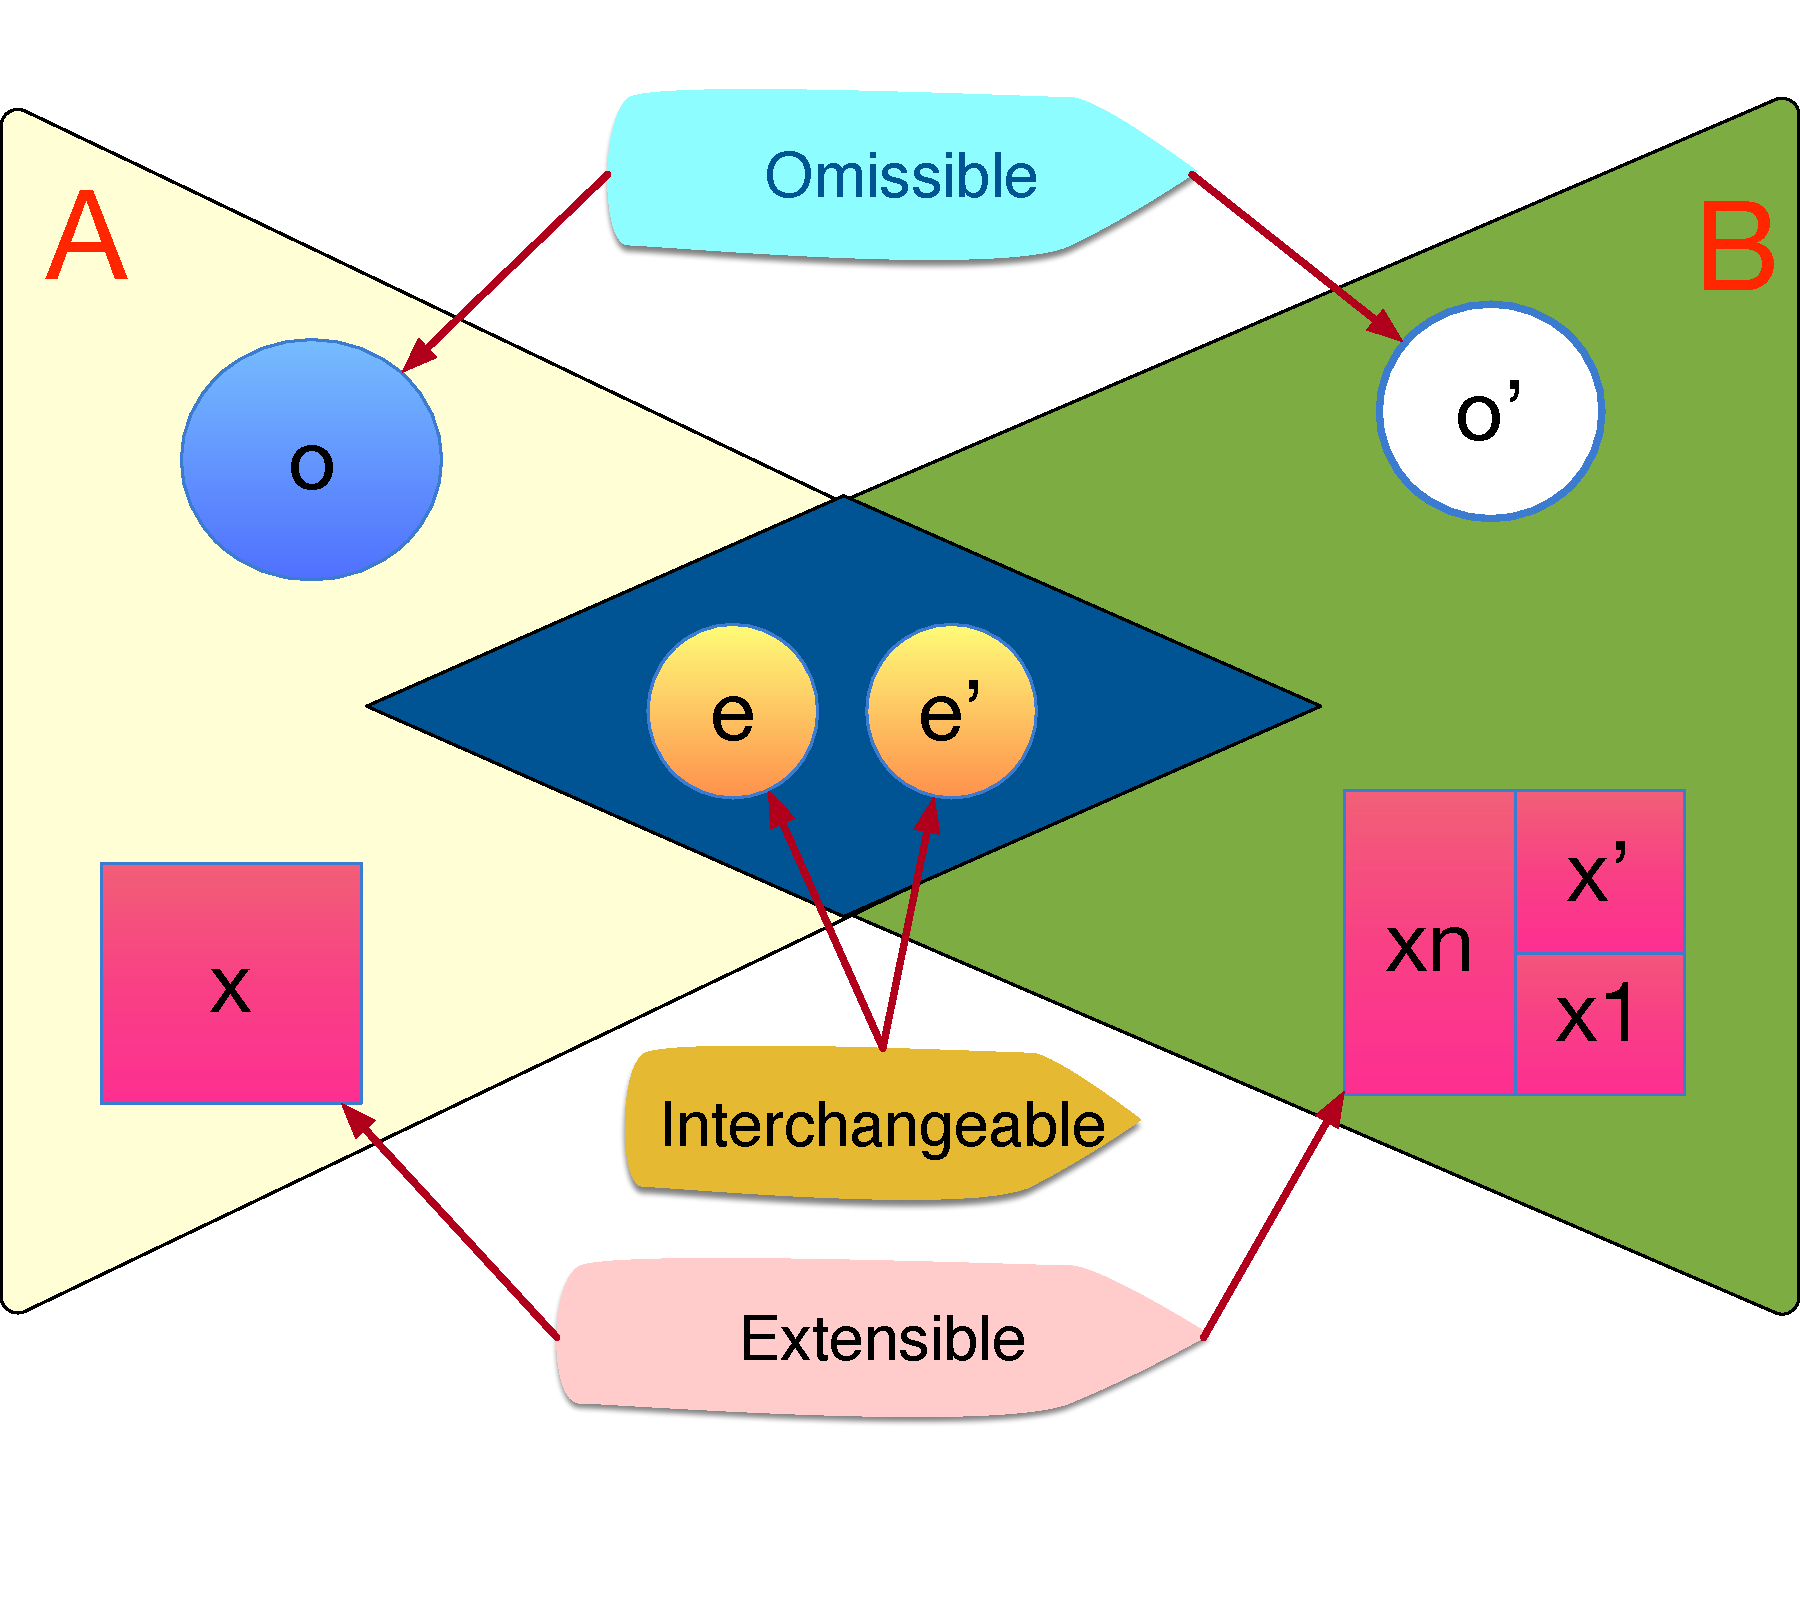
\includegraphics[width=3in]{ioe}
\caption{classifier elements into 3 types}
\label{fig:ioe}
\end{figure}

%AADL was born as an avionics-focused domain-specific language (DSL) and later on has been revised to represent and been used for a more general category of embedded real-time systems. SysML is an extension of the Unified Modeling Language (UML) intended to support system engineering and modeling. 
%We propose the ExSAM profile that extends SysML by adding AADL concepts to it with the goal of exploiting the key advantages of both languages in a seamless way. More precisely, by using ExSAM and any SysML modeling environment, we will be able to both model system engineering concepts and use AADL analysis tools where needed. We describe the ExSAM profile through several examples and compare it with existing alternatives. We have implemented ExSAM using IBM Rational Rhapsody and evaluated its completeness and usefulness through two case studies. Keywords: Integrated Control Systems (ICSs), Systems modeling languages, Architecture modeling languages, Embedded control systems, AADL, SysML.

 %Model-Driven Software Engineering (MDSE) provides suitable engines for defining, analyzing, and manipulating those models throughout the system development life cycle, including syntactical validation, model analysis, model simulation, model transformations, model execution, and model debugging [4]

%A pointcut which is a predicate  over a model that is used to select relevant model elements called join points. 2,an advice which is a new behavior meant to replace( or complement) the matched ones.\cite{Jezequel:2008ik}
%Our approach works at the high-level and early stage of development. 


%Therefore, there is a need for collaborative platforms to allow modelers to work together. We proposed a new approach to blending different languages seamlessly by manipulating metamodel with a set of transformation operators at the high-level and early stage of development. The process starts from a SysML system model, developed according to the platform-based design (PBD) paradigm, in which a functional model of the system (SW) is paired to a model of the execution platform (HW). Subsystems are refined as AADL models. In turn, AADL models are implemented as code and transfer to model-checker to perform verification and validation respectively. We illustrate our approach with an experimental of (engine??) design processes represented as scenarios.





%The conception of multi-view design has been proposed to respond to currently complex system's requirements. It relied on Model-driven engineering (MDE) with involving several modeling languages (such as SysML, AADL, etc.) and using principles of separation of concerns as well as domain-specific languages (DSL) to make stakeholders from diverse domains to work in a coordinated manner on different aspects of the system. It could help in reducing the gap between heterogeneous domains and making diverse expertise work together to produce a coherent and complete system. Therefore, there is a need for collaborative platforms to allow modelers to work together. We proposed a new approach to blending different languages seamlessly by manipulating metamodel on the high-level and early stage of development. Firstly, we are established in engineering framework (Capella) which adopts SysML as a modeling language. Furthermore, we proposed a set of transformation operators that can construct an interpretation system to translate designs into AADL develop environment (OASTE) automatically, and then it can refine models and performance verification and validation respectively. We illustrate our approach with an experimental of (engine??) design processes represented as scenarios.


%The process start from a SysML system model, developed according to the platform-based design (PBD) paradigm, in which a functional model of the system is paired to a model of the execution platform. Subsystems are refined as Simulink models or hand coded in C++. In turn, Simulink models are implemented as software code or firmware on FPGA, and an automatic generation of the implementation is obtained. Based on the SysML system architecture specification, our framework drives the generation of Simulink models with consistent interfaces, allows the automatic generation of the communication code among all subsystems (including the HW-FW interface code).

%The conception of multi-view design has been proposed to respond to currently complex system's requirements. It relied on Model-based approach (MBA) and involved several modeling languages (such as SysML, AADL, etc.). However, we are not able to integrate all of them into a mono design platform. Hence, we proposed a new approach to blending them seamlessly and extended their capabilities without extending development platform, that we named co-design operation. Firstly, we are established in engineering framework --Capella which adopts SysML as a modeling language. Furthermore, we proposed a set of transformation operators that can construct an interpretation system to automatically translate  Capella designs into AADL develop environment (OASTE), and then it can refine models and performance verification and validation respectively. We illustrate our approach with an experimental of (engine??) design processes represented as scenarios.





%developed according to the platform-based design (PBD) paradigm, in which a functional model of the system (SW) is paired to a model of the execution platform (HW). Subsystems are refined as AADL models. In turn, AADL models are implemented as code and transfer to model-checker to perform verification and validation respectively. We illustrate our approach with an experimental of (engine??) design processes represented as scenarios.


 
%The development of complex software-intensive systems requires stakeholders from diverse domains to work in a coordinated manner on different aspects of the system. Model-driven engineering (MDE) helps in reducing the gap between heterogeneous domains using principles of separation of concerns, automatic generation and domain-specific languages (DSL). MDE is thus a potential solution to help develop systems collaboratively. In MDE, stakeholders work on models in order to design, transform, simulate, and analyze systems. Teams of stakeholders with varying expertise work together to produce a coherent and complete system. Therefore, there is a need for collaborative platforms to allow modelers to work together.
%we present the different research projects we have been working on in the topic of collaborative modeling in MDE. After laying a set of necessary requirements I address several topics. We will look at the data structures needed to ensure near real-time collaboration. We will see how multi-view modeling is essential to let users work on different aspects of the system concurrently. Having users from different domains and expertise, we show how to adapt the modeling environment specifically to the needs and habits of the user. We will discuss automatic generation of restrictive modeling IDEs that can support all sorts of user interaction modes.